\chapter{自旋、同位旋、色與膠子自相互作用}

\section{以電動力學為類比理解量子色動力學}

量子色動力學的範圍太大，無法在一堂講座中完整介紹。這裡的目標是建立基本的直觀圖像，而非探討更深入的數學。

量子電動力學是描述電子與光子的理論，也是庫侖力的量子理論。如果把原子核視為固定的電場源，不探究它的運動或內部結構，那麼 QED 就是描述原子的理論。

量子色動力學對夸克與膠子也扮演類似的角色。它描述粒子本身、粒子之間的作用力，以及它們形成的複合物。這些複合物稱為\emph{強子}。質子和中子是重子：它們帶有淨夸克數，亦即非零的重子數。介子則由夸克--反夸克組成。重子和介子中也都含有膠子。

膠子不帶電，但它們提供束縛夸克所需的場。在這方面，膠子場所扮演的角色，類似於束縛原子的電磁場。

在介紹色與膠子之前，不妨先回顧自旋的數學。同一套數學幾乎直接再次出現在\emph{同位旋}中；色理論也呈現相關的模式。群論是這些構造的基礎，不過所需的概念可以從角動量出發來理解。

\section{角動量多重態}

角動量的各分量滿足
\begin{equation}
[L_x,L_y]=i\hbar L_z,
\end{equation}
以及循環置換後相應的關係
\begin{equation}
[L_y,L_z]=i\hbar L_x,
\qquad
[L_z,L_x]=i\hbar L_y.
\end{equation}
三個分量彼此不對易，因此無法同時測量。描述一個態時，必須選定一條軸；通常選\(z\)軸，並以沿該軸的角動量分量來標記各態。

這項選擇並未破壞自然界的旋轉對稱性；它只是在描述中選定一個方向，作為記錄狀態的基準。

\(z\)分量的允許值是量子化的，相鄰值相差一個\(\hbar\)。列出這些值時令\(\hbar=1\)，自旋為\(\ell\)的多重態包含
\begin{equation}
m=\ell,\ell-1,\ldots,-\ell.
\end{equation}
因此，獨立態的數目為
\begin{equation}
2\ell+1.
\end{equation}

前幾個多重態可以明確列如下：
\begin{align}
\ell=0:&\qquad m=0,\\
\ell=\frac12:&\qquad m=\frac12,-\frac12,\\
\ell=1:&\qquad m=1,0,-1,\\
\ell=\frac32:&\qquad
m=\frac32,\frac12,-\frac12,-\frac32,\\
\ell=2:&\qquad m=2,1,0,-1,-2.
\end{align}

就目前的討論而言，半整數自旋屬於費米子，整數自旋屬於玻色子。電子的自旋為\(\tfrac12\)。自旋為零的粒子完全沒有角動量。光子的自旋為一；原子和原子核也可以有自旋為一的態。原子和原子核同樣可以具有自旋\(\tfrac32\)，而這種計數方式也適用於更高自旋。

記號必須區分總自旋與自旋分量。\(\ell\)標記多重態，同時也是\(z\)分量可能達到的最大值；\(m\)則標記多重態中的特定態。因此，自旋為一的物體有三個態，自旋為\(\tfrac12\)的物體則有兩個態。

\section{兩個自旋為二分之一的粒子如何組合}

考慮兩個自旋為\(\tfrac12\)的粒子，並忽略它們的軌道角動量。它們的自旋直積空間有四個基底態：
\begin{equation}
|\uparrow\uparrow\rangle,\qquad
|\uparrow\downarrow\rangle,\qquad
|\downarrow\uparrow\rangle,\qquad
|\downarrow\downarrow\rangle.
\end{equation}
相應的\(z\)分量為
\begin{align}
|\uparrow\uparrow\rangle &: m=+1,\\
|\uparrow\downarrow\rangle &: m=0,\\
|\downarrow\uparrow\rangle &: m=0,\\
|\downarrow\downarrow\rangle &: m=-1.
\end{align}

兩個自旋都向上的態表明，自旋為一的多重態必定存在：最大\(z\)分量為\(+1\)。自旋為一的多重態只有三個態：
\begin{equation}
m=+1,\quad 0,\quad -1.
\end{equation}
然而，直積空間有四個態，其中包括兩個彼此獨立、\(m=0\)的態。它們不可能全都屬於同一個自旋為一的多重態。多出來的態也不可能是自旋為二，因為自旋為二的多重態需要五個態。因此，四個直積態必須分成三個自旋為一的態，以及一個自旋為零的態。

兩個\(m=0\)基底態的哪種組合屬於自旋為一的多重態？交換兩個粒子後，兩個自旋對齊的態保持不變：
\begin{equation}
|\uparrow\uparrow\rangle\longrightarrow|\uparrow\uparrow\rangle,
\qquad
|\downarrow\downarrow\rangle\longrightarrow|\downarrow\downarrow\rangle.
\end{equation}
相對地，兩個混合自旋的直積態會互換：
\begin{equation}
|\uparrow\downarrow\rangle
\longleftrightarrow
|\downarrow\uparrow\rangle.
\end{equation}
兩態相加後，在交換下保持對稱：
\begin{equation}
|\uparrow\downarrow\rangle+|\downarrow\uparrow\rangle.
\end{equation}
歸一化後須乘上\(1/\sqrt2\)：
\begin{equation}
|1,0\rangle
=
\frac{|\uparrow\downarrow\rangle
      +|\downarrow\uparrow\rangle}{\sqrt2}.
\end{equation}

\begin{figure}[h]
\centering
\includegraphics[width=0.78\textwidth]{lecture_02_figure_02.png}
\caption{對稱的混合自旋組合形成自旋三重態中的\(m=0\)態。}
\lectureframe{00:15:08}
\end{figure}

加上兩個自旋對齊的態，便得到自旋為一的三重態：
\begin{align}
|1,+1\rangle &=|\uparrow\uparrow\rangle,\\
|1,0\rangle &=
\frac{|\uparrow\downarrow\rangle
      +|\downarrow\uparrow\rangle}{\sqrt2},\\
|1,-1\rangle &=|\downarrow\downarrow\rangle.
\end{align}
另一個與它正交的組合帶有負號：
\begin{equation}
|0,0\rangle
=
\frac{|\uparrow\downarrow\rangle
      -|\downarrow\uparrow\rangle}{\sqrt2}.
\end{equation}
這個組合在交換下反對稱，形成只有一個態、總自旋為零的多重態。因此
\begin{equation}
\frac12\otimes\frac12=1\oplus0.
\end{equation}

這個對稱的混合自旋態具有\(m=0\)，但它\emph{並不}代表總角動量為零。它屬於自旋為一的三重態。旋轉座標軸時，它會與\(m=\pm1\)態混合。只有反對稱組合才有\(\ell=0\)。

就角動量而言，單態如同空無一物的空間。它仍可能帶有能量、電荷或其他量子數，但不帶角動量。

可以透過一個思想實驗檢驗這項區別。假設除了角動量守恆之外，其他守恆定律都不考慮，並問：哪一種雙粒子自旋態可以直接消失？兩個自旋對齊的態都不能消失，因為各自屬於自旋為一的多重態。對稱的\(m=0\)態也不能消失。雖然它的\(z\)分量為零，總自旋仍為一；相對於其他軸，它仍有非零的分量。只有反對稱單態可以在不違反角動量守恆的情況下消失。

\begin{classroomqa}
\audiencequestion{沿\(z\)軸測量這個對稱的混合自旋態，結果會是\(+1\)還是\(-1\)？\lecturetimestamp{00:19:28}}
\lecturerresponse{不會。沿\(z\)軸測量時，結果為零。不過，這個態的總自旋仍為一，因此沿另一條軸測量時，結果可能是\(+1\)或\(-1\)。}
\end{classroomqa}

\section{三個自旋為二分之一的粒子}

現在把三個自旋為\(\tfrac12\)的粒子組合起來。它們共有
\begin{equation}
2\times2\times2=8
\end{equation}
個直積態。如果三個自旋都向上，總\(z\)分量便是\(+\tfrac32\)。因此，必定存在自旋為\(\tfrac32\)的多重態，其中包含
\begin{equation}
2\left(\frac32\right)+1=4
\end{equation}
個態。

還剩下四個態。它們不可能構成另一個自旋為\(\tfrac32\)的多重態，因為\(m=\pm\tfrac32\)態已經用過了。剩餘態所能達到的最大分量只有\(+\tfrac12\)和\(-\tfrac12\)。三個半整數自旋也不可能合成總自旋為零。因此，剩餘態必定組成自旋為\(\tfrac12\)的多重態。

自旋為\(\tfrac12\)的多重態包含兩個態。既然還剩四個態，就表示有兩個不同的自旋為\(\tfrac12\)的多重態：
\begin{equation}
\frac12\otimes\frac12\otimes\frac12
=
\frac32\oplus\frac12\oplus\frac12.
\end{equation}
之後，當自旋向上與自旋向下這兩個態換成稱為上夸克和下夸克的兩種夸克味時，還會再看到同樣的模式。

\section{作為內部自旋的同位旋}

同位旋，又稱同位素自旋，是普通自旋的內部類比。普通自旋與物理空間的旋轉有關，同位旋則不是。它描述的是內部數學空間中的變換；該空間的兩個基本態將對應於
\begin{equation}
u,\qquad d.
\end{equation}
此處的\emph{上}和\emph{下}只是夸克味的標籤，與普通空間中的上下方向無關。

\editorialnote{從內部自旋空間的定義過渡到下一段強子質量尺度的論證時，有一小段內容無法有把握地還原，因此不據此推斷任何額外的物理主張。}

為什麼\(u\)和\(d\)適合用來類比？強子物理的典型能量尺度是數百 MeV。典型輕介子的質量是數百 MeV，而將三個夸克束縛成核子所涉及的能量也在相近尺度。相較之下，普通原子核的束縛能只有數 MeV。因此，質子和中子在原子核內受到束縛的作用力，是在遠小於夸克於強子內部所受束縛力的能量尺度上考慮的。

六種夸克味中，\(u\)和\(d\)相較於強子尺度而言很輕。產生重夸克需要更多能量，含有重夸克的強子也可能衰變成較輕的強子。因此，最穩定的輕強子由上夸克和下夸克組成。

下夸克比上夸克重；依照這裡採用的估算，質量約為上夸克的兩倍。不過，兩者的質量相較於數百 MeV 都很小。第一階近似下，在強子尺度上可將兩者都視為近乎無質量。更重要的是，兩者的質量可視為近乎相等。

這種近似相等帶來一種對稱性。若交換上夸克和下夸克，強相互作用的物理情況幾乎不變。質子
\begin{equation}
p\sim uud,
\end{equation}
和中子
\begin{equation}
n\sim udd,
\end{equation}
就是最簡單的例子：兩者只差在\(u\)和\(d\)互換，質量也非常接近。

因此，交換
\begin{equation}
u\longleftrightarrow d
\end{equation}
在數學上的處理方式，類似於
\begin{equation}
|\uparrow\rangle\longleftrightarrow|\downarrow\rangle.
\end{equation}
對普通自旋而言，這種變換相當於旋轉空間中的一條軸；對同位旋而言，則是內部空間中的旋轉。兩者的數學形式類似，物理意義卻不同。

\begin{figure}[h]
\centering
\includegraphics[width=0.80\textwidth]{lecture_02_figure_03.png}
\caption{兩個自旋為\(\tfrac12\)的態分解為三重態與單態；這是相應同位旋構造的模型。}
\lectureframe{00:27:42}
\end{figure}

字首\emph{iso}源自\emph{isotope}。早期的核物理描述把質子和中子視為同一個內部二重態的兩個成員。在原子核中交換質子和中子，會使一種同位素變成另一種。夸克模型後來將質子與中子的互換，追溯到底層\(u\)和\(d\)的互換。

\begin{classroomqa}
\audiencequestion{同位旋是否早於夸克模型提出？\lecturetimestamp{00:30:19}}
\lecturerresponse{是。同位旋在夸克提出之前就已引入，歷史上與海森堡有關。夸克模型後來賦予它\(u\)與\(d\)夸克味的詮釋。}
\end{classroomqa}

同位旋並非自然界的精確對稱性。上夸克和下夸克的質量並不完全相等，電荷也不同：
\begin{equation}
Q(u)=+\frac23,
\qquad
Q(d)=-\frac13.
\end{equation}
即使兩者質量相等，電磁作用仍會將它們區分開來。

在較小的強子和核系統中，電磁效應相較於強相互作用很弱。在大型原子核中，電荷間的排斥可能變得重要；但對質子、中子，或氦這類小型原子核而言，相較於強相互作用的尺度，電磁效應只是較小的修正。因此，同位旋近似包含兩個步驟：

\begin{enumerate}
\item 忽略\(u\)--\(d\)的質量差；
\item 關閉兩者之間的電磁差異，只保留強相互作用。
\end{enumerate}

在這項近似下，\(u\)和\(d\)之間的變換，在數學上便成為類似普通自旋對稱性的對稱變換。

\section{核子同位旋二重態}

單一夸克無法被孤立，作為自由的實驗室對象加以觀察。最簡單的已觀測重子由三個夸克組成。因此，三個自旋的計數方式有直接的同位旋類比：三個同位旋為\(\tfrac12\)的夸克，可以合成總同位旋為\(\tfrac32\)或\(\tfrac12\)的態。

先看總同位旋為\(\tfrac12\)的情況。這種多重態有
\begin{equation}
2\left(\frac12\right)+1=2
\end{equation}
個態，分別是質子和中子：
\begin{equation}
p\sim uud,
\qquad
n\sim udd.
\end{equation}
它們的電荷為
\begin{align}
Q(p)
&=\frac23+\frac23-\frac13
=+1,\\
Q(n)
&=\frac23-\frac13-\frac13
=0.
\end{align}
交換\(u\)與\(d\)，質子與中子也會互換。兩者構成同位旋為\(\tfrac12\)的二重態。

為了討論交換對稱性，暫時以\(1,2,3\)標記三個夸克槽位。這些標記不代表固定的夸克位置，因為夸克會運動。一個示意性的質子因子為
\begin{equation}
d_1\bigl(u_2u_3-u_3u_2\bigr).
\end{equation}

\begin{figure}[h]
\centering
\includegraphics[width=0.58\textwidth]{lecture_02_figure_04.png}
\caption{示意性質子態中，經反對稱化的兩夸克\(u\)因子。}
\lectureframe{00:35:43}
\end{figure}

這個表示式旨在凸顯費米子的交換反對稱性，並非完整的質子波函數。完整的態必須結合味、普通自旋、空間依賴性，以及---即將變得不可或缺的---色。

\editorialnote{下標只是暫時使用的槽位或單粒子標記。兩個相同的\(u\)味態並未構成通常所說的反對稱同位旋單態，因此，單憑這個因子不能推論同位旋為零。保留這個表示式，只是為了呈現局部的槽位反對稱化步驟；質子的總同位旋則由完整的三夸克態決定。}

與先前自旋構造的有限類比在於，量子態可以依照標記的交換，對稱或反對稱地組合。但光憑這項類比，無法判定所示\(uu\)因子的同位旋。

質子具有普通自旋\(\tfrac12\)，也具有同位旋\(\tfrac12\)。中子亦然。兩者是不同的量子數：普通自旋與物理空間的旋轉有關，同位旋則涉及\(u\)--\(d\)內部對稱性。

\section{Delta 四重態}

三個輕夸克也能形成總同位旋為\(\tfrac32\)的態，構成四態多重態，也就是 Delta 四重態：
\begin{equation}
\begin{aligned}
\Delta^{++}&\sim uuu,
&
\Delta^{+}&\sim uud,
\\
\Delta^{0}&\sim udd,
&
\Delta^{-}&\sim ddd.
\end{aligned}
\end{equation}
Delta 態的普通自旋為\(\tfrac32\)，同位旋為\(\tfrac32\)。在分量最大的態中，三個普通自旋彼此平行，三個同位旋分量也彼此平行。

僅憑\(uud\)這樣的夸克組成，無法判定該態是質子還是\(\Delta^+\)。相同的夸克味組合，可以構成總自旋和總同位旋不同的態。

\begin{classroomqa}
\audiencequestion{Delta 四重態中的\(uud\)態與質子有何不同？\lecturetimestamp{00:41:08}}
\lecturerresponse{兩者的普通自旋不同：質子的自旋為\(\tfrac12\)，Delta 態的自旋則為\(\tfrac32\)。夸克組成的總同位旋態也不同。}
\end{classroomqa}

\begin{classroomqa}
\audiencequestion{Delta 四重態中間的成員是同位旋為\(\tfrac12\)的態嗎？\lecturetimestamp{00:41:52}}
\lecturerresponse{不是。它們的同位旋分量是\(+\tfrac12\)和\(-\tfrac12\)，但總同位旋仍是\(\tfrac32\)。總同位旋為\(\tfrac32\)的多重態必定包含四個分量態。}
\end{classroomqa}

四個同位旋分量對應於
\begin{equation}
I_3=\frac32,\frac12,-\frac12,-\frac32.
\end{equation}
它們的電荷為
\begin{align}
Q(\Delta^{++})&=+2,\\
Q(\Delta^{+})&=+1,\\
Q(\Delta^{0})&=0,\\
Q(\Delta^{-})&=-1.
\end{align}
中間兩個態的電荷恰好與質子和中子相同，但它們仍是不同的態，因為自旋與同位旋的耦合方式不同。

近似同位旋對稱性使四個 Delta 的質量幾乎相等。\(u\)--\(d\)質量差很小，因此只會造成四重態內微小的質量分裂。Delta 的共同質量尺度約為
\begin{equation}
m_\Delta\sim1200\,\mathrm{MeV},
\end{equation}
質子和中子的質量則接近
\begin{equation}
m_N\sim940\,\mathrm{MeV}.
\end{equation}

\subsection{\texorpdfstring{\(\Delta^{++}\)}{Delta++}的衰變}

Delta 態的質量足以讓它衰變成一個核子和一個{\proseunicodefont π}介子。考慮
\begin{equation}
\Delta^{++}\sim uuu.
\end{equation}
當組成粒子分開時，可以產生一對夸克--反夸克。若嘗試插入\(u\bar u\)，末態就會留下含三個\(u\)夸克的重子；在可用能量下，這無法構成較輕且允許的衰變道。若改為產生一對\(d\bar d\)，各組成粒子便可重新組合成
\begin{equation}
uuu+d\bar d
\longrightarrow
uud+u\bar d.
\end{equation}
兩個末態複合粒子分別是
\begin{equation}
uud=p,
\qquad
u\bar d=\pi^+,
\end{equation}
因此
\begin{equation}
\Delta^{++}\longrightarrow p+\pi^+.
\end{equation}

\begin{figure}[h]
\centering
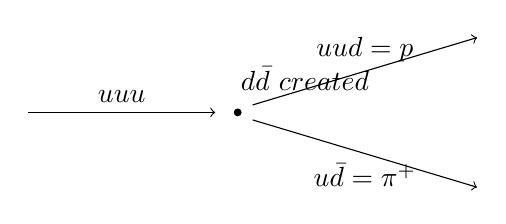
\begin{tikzpicture}[scale=0.95]
\draw[->] (-3,0) -- (-0.5,0) node[midway,above] {$uuu$};
\fill (-0.2,0) circle (1.5pt);
\draw[->] (0,0.1) -- (3,1.0) node[midway,above] {$uud=p$};
\draw[->] (0,-0.1) -- (3,-1.0) node[midway,below] {$u\bar d=\pi^+$};
\node at (0.7,0.45) {$d\bar d\ \text{created}$};
\end{tikzpicture}
\caption{衰變\(\Delta^{++}\rightarrow p+\pi^+\)中的組成粒子重新組合。}
\end{figure}

電荷守恆一目了然：
\begin{equation}
Q(p)+Q(\pi^+)=1+1=2=Q(\Delta^{++}).
\end{equation}
粗略的質量平衡也允許這項衰變：
\begin{equation}
1200\,\mathrm{MeV}
>
940\,\mathrm{MeV}+140\,\mathrm{MeV}.
\end{equation}
末態還有足夠的剩餘能量轉化為動能。

四種 Delta 態都可以衰變成質子或中子與一個{\proseunicodefont π}介子。它們的壽命極短。若以光穿越一個質子所需的時間來估算，便可得到其數量級：
\begin{equation}
\tau_\Delta
\sim
\frac{10^{-13}\,\mathrm{cm}}
     {10^{10}\,\mathrm{cm/s}}
\sim10^{-23}\,\mathrm{s}.
\end{equation}
儘管如此，它們仍能存續足夠長的時間，使我們得以在粒子碰撞中辨認出這些不同的粒子。

\begin{classroomqa}
\audiencequestion{在這種組成粒子的記帳方式中，\(u\)和\(d\)符號的書寫順序重要嗎？\lecturetimestamp{00:48:49}}
\lecturerresponse{就目前的討論而言，順序並不重要。重要的是夸克味的組成，以及完整量子態的組合方式。}
\end{classroomqa}

\section{泡利難題與色的必要性}

\(\Delta^{++}\)凸顯了一個矛盾。它由三個上夸克組成。在自旋為\(\tfrac32\)的態中，三個夸克的普通自旋可以全部平行。它們的同位旋也相同，因為全都是\(u\)。如果自旋、夸克味和最低能量空間態就構成完整描述，那麼這三個夸克便是完全相同的費米子，並佔據同一個態。泡利不相容原理禁止這種情況。

\begin{classroomqa}
\audiencequestion{如果重複出現的上夸克看似佔據同一個態，它們怎麼會是費米子？\lecturetimestamp{00:48:58}}
\lecturerresponse{它們不可能在所有量子數上都完全相同。\(\Delta^{++}\)顯示夸克除了普通自旋、夸克味和空間態之外，還需要一個額外標籤；這個標籤就是色。}
\end{classroomqa}

這個新標籤有三種可能值：
\begin{equation}
r,\qquad g,\qquad b,
\end{equation}
分別稱為紅、綠、藍。這些名稱與可見的顏色無關，只是三種內部態的任意稱呼。也可以使用其他名稱；重要的是有三種不同的可能態。

同一種夸克味的紅、綠、藍三種色態，質量與一般可觀測性質都相同，但仍是不同的量子態。因此，\(\Delta^{++}\)可以由一個紅色的\(u\)、一個綠色的\(u\)和一個藍色的\(u\)組成，讓三個費米子不再佔據完全相同的態。

六種夸克味為
\begin{equation}
u,\ d,\ c,\ s,\ t,\ b.
\end{equation}
這個排列順序並非依質量排列。上夸克最輕，其次是下夸克。粲夸克比奇夸克重得多，頂夸克則比底夸克重得多。每種夸克味都有三種色態，因此夸克至少帶有兩種不同的內部標籤：
\begin{equation}
\text{flavor}\quad\text{and}\quad\text{color}.
\end{equation}

能不能用位置或動量來區分這三個夸克？Delta 難題涉及的是最低能量態；在這種態中，空間與動量結構無法在不改變能量和對稱性質的情況下，提供三種不同的標籤。因此，缺少的區分必須來自新的內部自由度。

自旋在原子物理中的作用，提供了一個有啟發性的類比。兩個看似佔據同一軌域態的電子，仍可因自旋態不同而有所區別。同樣地，夸克即使具有相同的夸克味、普通自旋和空間態，仍可因色不同而有所區別。

\editorialnote{氦光譜學、泡利原理，以及烏倫貝克和古茲密特之間的精確歷史脈絡，已明確標示為無法確定。此處保留這個類比，但不宣稱這就是自旋發現的確切先後順序。}

南部陽一郎因指出夸克需要這種額外自由度而受到關注。名稱不影響物理要點：三種夸克色態化解了泡利矛盾。這裡相關的是泡利原理，而非海森堡不確定性原理。

\editorialnote{\emph{色}一詞的確切由來和後續歷史尚不確定，因此此處不提出更明確的年代說法。口述中提及的海森堡不確定性原理，依照此處關於費米子統計的論證，更正為泡利不相容原理。}

同樣的色構造也適用於質子和中子。它們的態並非把每個夸克味符號固定指定為某一種色而構成。物理重子是所有允許的紅、綠、藍配置所形成的量子疊加，並具備適當的交換對稱性。

\begin{classroomqa}
\audiencequestion{色是能直接測量的一般物理性質嗎？\lecturetimestamp{00:56:55}}
\lecturerresponse{三種色態的質量與一般性質都相同。它們的差異會透過允許的組合和碰撞過程，以相互關係的方式呈現。實驗顯示確實存在三種不同的色態，但我們無法製備孤立的帶色夸克來直接檢驗。}
\end{classroomqa}

\begin{classroomqa}
\audiencequestion{色守恆嗎？\lecturetimestamp{00:57:38}}
\lecturerresponse{是。色守恆，但這裡討論的可觀測粒子都不帶色，因此這項守恆定律看起來有些特殊。}
\end{classroomqa}

\editorialnote{更精確地說，漸近態強子都是色單態。所謂``不帶色''，並不是把紅、綠、藍以數值相加而得出的阿貝爾淨荷。}

\begin{classroomqa}
\audiencequestion{僅有\(uud\)夸克的質子，真的需要三種色態嗎？似乎只要區分兩個\(u\)夸克就夠了。\lecturetimestamp{00:57:58}}
\lecturerresponse{這個例子確實顯示需要某種額外區分，但不能據此斷定必須有三種。\(\Delta^{++}\)則明確顯示需要三個不同標籤：其中三個上夸克的普通自旋彼此平行，同位旋也彼此平行。}
\end{classroomqa}

這就是 Delta 如此重要的原因。質子和中子的自旋及夸克味對稱性較複雜，矛盾可能被波函數的細節掩蓋。在\(\Delta^{++}\)中，矛盾則一目了然：
\begin{equation}
uuu,\qquad
\uparrow\uparrow\uparrow,
\qquad
\text{one lowest spatial state}.
\end{equation}
因此需要一個有三種取值的新標籤。強子碰撞資料也獨立證實了三種色態的存在。

即使對稱性標籤的不同取值單獨看來彼此等價，它仍可能具有意義。未選定空間軸時，兩種自旋方向在物理上等價；另一個物體可以提供參考軸，顯示它們之間的關係。類似地，質子或中子會在同位旋空間中選定一個方向；與其他態比較，就能看出內部取向彼此平行或反平行。色的情況更微妙，但其物理內容同樣透過關係、關聯性及交互作用規則呈現，而非透過可見的顏色。

也可以設想放棄泡利原理，但那就需要新的數學架構：普通量子場論把粒子分為費米子或玻色子，並沒有已確立的第三種選項能解決這個問題。QCD 保留夸克的費米子性質，並引入色。

\begin{classroomqa}
\audiencequestion{泡利原理要求的這種隱藏區分，對應到什麼可觀測量？\lecturetimestamp{01:01:08}}
\lecturerresponse{這個問題遠比熟悉的位置、動量或同位旋可觀測量微妙。完整解答需要進一步理解色動力學，因此留待後續討論。}
\end{classroomqa}

\begin{classroomqa}
\audiencequestion{夸克具有費米子性質，是從強子的自旋指派推論出來的嗎？\lecturetimestamp{01:01:43}}
\lecturerresponse{是。}
\end{classroomqa}

\editorialnote{前兩個聽眾問題的部分措辭無法辨認。問題主旨和簡短回答都可以確認，但無法據此推定更詳細的說法。}

\begin{classroomqa}
\audiencequestion{如何將特定的色指定給質子中的某個夸克？\lecturetimestamp{01:01:55}}
\lecturerresponse{我們不會把固定的色指定給一個可永久辨認的組成夸克。質子是所有允許的紅、綠、藍配置所形成的量子疊加，其中自旋、夸克味、空間和色因子都依適當方式對稱化或反對稱化。\(\Delta^{++}\)很有用，因為它平行的自旋和夸克味結構，清楚顯示出色的必要性，而不必先寫出完整的質子波函數。}
\end{classroomqa}

色在 QCD 中的角色，類似電荷在電動力學中的角色：它是決定交互作用的量子數。QCD 能非常精確地描述強子碰撞的實驗資料。這套理論架構最終仍須由其推論是否符合實驗來驗證。

\section{光子與膠子}

夸克是量子色動力學中的費米子物質粒子，在這個有限的意義上類似量子電動力學中的電子。是什麼力量將它們束縛在一起？

在電動力學中，電子是電磁場的源。以粒子的語言來說，電子會發射和吸收光子；光子在帶電粒子之間交換，因而產生作用力。夸克同樣是膠子場的源，也能發射和吸收膠子。

膠子在幾個重要方面與光子相似。它們是無質量、自旋為一的粒子，具有類似光子的偏振態；動量和偏振則是一般的動力學性質。關鍵差異在於，膠子攜帶色資訊，因此彼此也會相互作用。

光子不帶電荷。在量子電動力學的基本層次，一個光子不會發射另一個光子，兩束光也會彼此穿過而不相互作用。雖然存在涉及電子迴圈、效應極微小的高階光子—光子相互作用，但那是次級效應，並非光子的直接自耦合。在真空中，量子電動力學的基本頂點只是電子發射或吸收光子。

\begin{figure}[h]
\centering
\begin{tikzpicture}[scale=1.0]
\draw[->] (-2,-1) -- (0,0);
\draw[->] (0,0) -- (2,-1);
\draw[smooth] plot coordinates {
(0,0) (0.16,0.27) (0.32,0.23) (0.48,0.52)
(0.64,0.48) (0.80,0.77) (0.96,0.73)
(1.12,1.02) (1.28,0.98) (1.44,1.27)
(1.60,1.23) (1.76,1.52)
};
\node at (-1.25,-0.75) {$e^-$};
\node at (1.25,-0.75) {$e^-$};
\node at (1.95,1.62) {$\gamma$};
\fill (0,0) circle (1.5pt);
\end{tikzpicture}
\caption{量子電動力學的基本頂點：電子發射或吸收光子。}
\end{figure}

反轉費米子線的方向，就會把電子的詮釋轉為正電子的詮釋。發射、吸收，以及經交叉變換得到的正電子過程，都是同一個頂點的不同排列方式。

為了記帳，可以姑且把光子想成具有電子--正電子對的某些性質。這個粒子對是電中性的；電子和正電子的自旋若方向對齊，總自旋可以是自旋一。在外部交互作用提供所需能量和動量時，光子可以產生電子--正電子對。這並不表示光子真的是由電子和正電子構成的。這種虛構粒子對的圖像對量子電動力學本身幫助不大，但它在量子色動力學中的顏色類比很有用。

\section{膠子的顏色--反顏色標記}

將夸克的三種顏色態表示為一個直欄：
\begin{equation}
q=
\begin{pmatrix}
r\\
g\\
b
\end{pmatrix}.
\end{equation}
將相應的反夸克標記表示為一個橫列：
\begin{equation}
\bar q=
\begin{pmatrix}
\bar r&\bar g&\bar b
\end{pmatrix}.
\end{equation}

膠子並不是夸克--反夸克束縛態。不過，在顏色記帳上，它的表現就像同時帶有一種顏色和一種反顏色。因此，各種可能的標記可以排列如下：
\begin{equation}
\begin{pmatrix}
r\bar r&r\bar g&r\bar b\\
g\bar r&g\bar g&g\bar b\\
b\bar r&b\bar g&b\bar b
\end{pmatrix}.
\end{equation}
乍看之下，這會得到九種組合。

\begin{classroomqa}
\audiencequestion{對角線上的顏色--反顏色項彼此無法區分嗎？\lecturetimestamp{01:13:37}}
\lecturerresponse{不能這麼簡單地說。對角線上的項彼此不同；關鍵在於，它們的總和不是獨立的量子態。}
\end{classroomqa}

實際上只有八種獨立的膠子態。三個對角線標記並非彼此無法區分，但特定的對角線總和
\begin{equation}
r\bar r+g\bar g+b\bar b
\end{equation}
並不構成量子色動力學中另一種獨立的膠子。至於這種簡化背後更深一層的原因，留待之後說明。就目前的顏色流討論而言，使用這九種表面上可能的標記很方便，只要記得其中一種對角線組合並不存在即可。

\section{夸克--膠子頂點}

夸克可以發射膠子，並以相同或不同的顏色離開。如果夸克帶著顏色\(a\)進入，並以顏色\(b\)離開，發射出的膠子就帶有記帳標記\(a\bar b\)：
\begin{equation}
a\longrightarrow b+(a\bar b).
\end{equation}
例如：
\begin{equation}
r\longrightarrow g+(r\bar g).
\end{equation}
紅色線延續到膠子中；綠色線則穿過出射夸克繼續延伸，並在膠子中反向延續為反綠色線。

夸克不一定要改變顏色。同一條規則也允許：
\begin{equation}
r\longrightarrow r+(r\bar r),
\end{equation}
或
\begin{equation}
r\longrightarrow b+(r\bar b).
\end{equation}

\begin{figure}[h]
\centering
\begin{tikzpicture}[scale=1.0]
\draw[->] (-2,-0.8) -- (0,0) node[midway,above] {$r$};
\draw[->] (0,0) -- (2,0.9) node[midway,above] {$g$};
\draw[smooth] plot coordinates {
(0,0) (0.20,-0.23) (0.40,-0.17) (0.60,-0.46)
(0.80,-0.40) (1.00,-0.69) (1.20,-0.63)
(1.40,-0.92) (1.60,-0.86) (1.80,-1.15)
(2.00,-1.09)
};
\node at (2.35,-1.12) {$r\bar g$};
\fill (0,0) circle (1.5pt);
\end{tikzpicture}
\caption{紅色夸克發射一個\(r\bar g\)膠子後變成綠色。}
\end{figure}

這是量子色動力學的一個基本組成單元。

\begin{classroomqa}
\audiencequestion{只有夸克改變顏色時，才會發射膠子嗎？\lecturetimestamp{01:17:15}}
\lecturerresponse{不會。出射夸克的顏色可以相同，也可以不同。無論哪種情況，發射出的膠子所帶的顏色--反顏色標記都會使顏色線保持連續。}
\end{classroomqa}

\section{三膠子頂點}

量子色動力學還有另一種基本交互作用，在量子電動力學中沒有基本對應。膠子可以直接與其他膠子相互作用。

先從一個\(r\bar b\)膠子開始。以顏色流的語言來說，它可以分裂成：
\begin{equation}
r\bar b
\longrightarrow
r\bar g+g\bar b.
\end{equation}
紅線延續為\(r\bar g\)，反藍線延續為\(g\bar b\)，而綠—反綠這一對則接合兩個出射膠子。這就構成三膠子頂點。

\begin{figure}[h]
\centering
\begin{tikzpicture}[scale=1.0]
\draw[smooth] plot coordinates {
(-2,0) (-1.80,0.12) (-1.60,-0.02) (-1.40,0.12)
(-1.20,-0.02) (-1.00,0.12) (-0.80,-0.02)
(-0.60,0.12) (-0.40,-0.02) (-0.20,0.12) (0,0)
};
\draw[smooth] plot coordinates {
(0,0) (0.20,0.27) (0.40,0.21) (0.60,0.50)
(0.80,0.44) (1.00,0.73) (1.20,0.67)
(1.40,0.96) (1.60,0.90) (1.80,1.19) (2.00,1.13)
};
\draw[smooth] plot coordinates {
(0,0) (0.20,-0.27) (0.40,-0.21) (0.60,-0.50)
(0.80,-0.44) (1.00,-0.73) (1.20,-0.67)
(1.40,-0.96) (1.60,-0.90) (1.80,-1.19) (2.00,-1.13)
};
\node at (-2.45,0) {$r\bar b$};
\node at (2.45,1.18) {$r\bar g$};
\node at (2.45,-1.18) {$g\bar b$};
\fill (0,0) circle (1.5pt);
\end{tikzpicture}
\caption{三膠子顏色流：\(r\bar b\rightarrow r\bar g+g\bar b\)。}
\end{figure}

不必把每一種允許的組合都背下來。沿著圖中的每條顏色線追蹤即可。若費米子線的時間方向反轉，就將它重新詮釋為相應的反粒子線或反顏色線。

\section{膠子交換與作用力}

膠子透過交換產生作用力，就像光子在帶電粒子之間交換時會產生電磁力一樣。

例如，藍夸克和反藍反夸克可以交換一個\(g\bar b\)膠子，之後分別變成綠夸克和反綠反夸克。符合兩個頂點的顏色流配置是\footnote{淨顏色變化\(b+\bar b\longrightarrow g+\bar g\)很清楚，但局部顏色標記曾經多次修正。藉由要求兩個頂點的顏色流都連續，可以重建交換膠子的標記\(g\bar b\)。}
\begin{equation}
b+\bar b
\longrightarrow
g+\bar g.
\end{equation}
在反夸克頂點處：
\begin{equation}
\bar b\longrightarrow\bar g+(g\bar b),
\end{equation}
而在夸克頂點處：
\begin{equation}
b+(g\bar b)\longrightarrow g.
\end{equation}
交換的膠子將顏色變化從一條費米子線傳到另一條。

\begin{figure}[h]
\centering
\begin{tikzpicture}[scale=1.0]
\draw[->] (-1.8,0) -- (-1.8,-1.8) node[midway,left] {$\bar b$};
\draw[->] (-1.8,1.8) -- (-1.8,0) node[midway,left] {$\bar g$};
\draw[->] (1.8,-1.8) -- (1.8,0) node[midway,right] {$b$};
\draw[->] (1.8,0) -- (1.8,1.8) node[midway,right] {$g$};
\draw[smooth] plot coordinates {
(-1.8,0) (-1.50,0.13) (-1.20,-0.03) (-0.90,0.13)
(-0.60,-0.03) (-0.30,0.13) (0,-0.03)
(0.30,0.13) (0.60,-0.03) (0.90,0.13)
(1.20,-0.03) (1.50,0.13) (1.8,0)
};
\node at (0,0.42) {$g\bar b$};
\fill (-1.8,0) circle (1.5pt);
\fill (1.8,0) circle (1.5pt);
\end{tikzpicture}
\caption{交換一個\(g\bar b\)膠子，使藍--反藍粒子對變成綠--反綠粒子對；反夸克的箭頭方向與時間增加的方向相反。}
\end{figure}

相同的交互作用也允許膠子之間產生作用力。一種自洽的實現方式是\footnote{本講說明了膠子之間的膠子交換，以及沿著線追蹤的規則，但圖中的局部標記曾經多次修正。圖中展示的配置符合最終的規則，並非對每個中間標記都能可靠還原的逐步記錄。}
\begin{equation}
(r\bar b)+(b\bar r)
\longrightarrow
(r\bar g)+(g\bar r),
\end{equation}
其中兩個外部膠子之間交換一個\(g\bar b\)膠子：
\begin{align}
r\bar b&\longrightarrow r\bar g+g\bar b,\\
b\bar r+g\bar b&\longrightarrow g\bar r.
\end{align}

\begin{figure}[h]
\centering
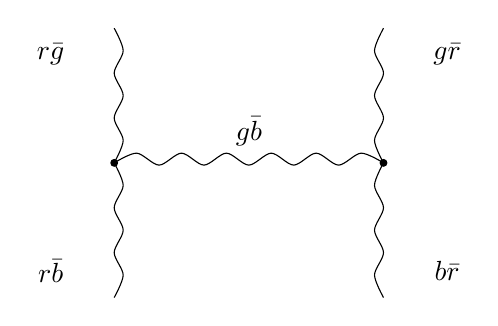
\begin{tikzpicture}[scale=0.95]
\draw[smooth] plot coordinates {
(-1.8,-1.8) (-1.68,-1.50) (-1.80,-1.20) (-1.68,-0.90)
(-1.80,-0.60) (-1.68,-0.30) (-1.8,0)
};
\draw[smooth] plot coordinates {
(-1.8,0) (-1.68,0.30) (-1.80,0.60) (-1.68,0.90)
(-1.80,1.20) (-1.68,1.50) (-1.8,1.8)
};
\draw[smooth] plot coordinates {
(1.8,-1.8) (1.68,-1.50) (1.80,-1.20) (1.68,-0.90)
(1.80,-0.60) (1.68,-0.30) (1.8,0)
};
\draw[smooth] plot coordinates {
(1.8,0) (1.68,0.30) (1.80,0.60) (1.68,0.90)
(1.80,1.20) (1.68,1.50) (1.8,1.8)
};
\draw[smooth] plot coordinates {
(-1.8,0) (-1.50,0.13) (-1.20,-0.03) (-0.90,0.13)
(-0.60,-0.03) (-0.30,0.13) (0,-0.03)
(0.30,0.13) (0.60,-0.03) (0.90,0.13)
(1.20,-0.03) (1.50,0.13) (1.8,0)
};
\node at (-2.65,-1.45) {$r\bar b$};
\node at (-2.65,1.45) {$r\bar g$};
\node at (2.65,-1.45) {$b\bar r$};
\node at (2.65,1.45) {$g\bar r$};
\node at (0,0.42) {$g\bar b$};
\fill (-1.8,0) circle (1.5pt);
\fill (1.8,0) circle (1.5pt);
\end{tikzpicture}
\caption{兩個膠子之間交換一個\(g\bar b\)膠子；每條顏色線和反顏色線都連續穿過各個頂點。}
\end{figure}

\section{膠子自相互作用與非線性場}

膠子的自相互作用改變了量子色動力學的性質。夸克可以透過交換膠子彼此束縛而形成強子；膠子也可以透過交換膠子彼此束縛。因此，量子色動力學中可能存在完全由膠子自由度構成、不含夸克的複合物。量子電動力學中則沒有僅由光子構成的對應基本束縛態。

用場的語言描述，也會得到相同結論。在基本層次上，真空中的兩列電磁波會彼此穿過。兩列膠子波則會相互作用、彼此形變。甚至同一個膠子場組態的不同部分也能彼此施力。因此，膠子場是非線性的。

\begin{classroomqa}
\audiencequestion{圖的兩側必須各自有相同數目的紅、綠、藍標記嗎？\lecturetimestamp{01:24:59}}
\lecturerresponse{實用的規則是沿著圖中的每條顏色線追蹤。這種連續性就是色荷守恆。如果費米子線在時間方向上折返，其標記就要改為相應的反粒子或反顏色標記。}
\end{classroomqa}

\begin{classroomqa}
\audiencequestion{圖的第一個版本中，所有顏色和反顏色標記都一致嗎？\lecturetimestamp{01:26:00}}
\lecturerresponse{不一致。有幾個標記需要修正。在一致的配置中，紅線、反藍線和綠線各自連續穿過頂點；反轉的費米子箭頭則詮釋為反粒子。}
\end{classroomqa}

\begin{classroomqa}
\audiencequestion{中間的膠子線是當作夸克--反夸克對來處理嗎？\lecturetimestamp{01:27:58}}
\lecturerresponse{只是在顏色記帳上如此。膠子並非字面意義上的夸克--反夸克複合態，但它帶有相應的顏色和反顏色性質。}
\end{classroomqa}

到目前為止，基本規則可以簡要歸納如下：

\begin{itemize}
\item 夸克會發射和吸收膠子；
\item 膠子會直接與其他膠子相互作用；
\item 每條顏色線和反顏色線都必須連續穿過頂點；
\item 沿時間方向反轉費米子線時，它會變成相應的反粒子線。
\end{itemize}

\begin{classroomqa}
\audiencequestion{以這些顏色--反顏色線來表示時，膠子仍然是無質量的嗎？\lecturetimestamp{01:28:13}}
\lecturerresponse{是的，膠子仍然無質量。接下來的限定談的是如何理解強子內夸克的質量。}
\end{classroomqa}

接下來要談禁閉和強子結構：為什麼從未觀察到孤立的色，以及夸克和膠子如何組成複合粒子。首先，先釐清組分夸克的質量是什麼意思。

\section{探測尺度與夸克質量的意義}

想像有個質量為\(m\)的小物體，附著在一塊柔軟、可變形的材料上---，例如一塊垂下來的口香糖。施加一個非常輕柔的力，並緩慢到讓柔軟材料有時間調整，使整個系統一起運動。此時測得的慣性，就是小物體與附著材料的慣性之和。

現在以非常高的頻率搖動這個小物體。柔軟材料來不及跟上快速運動，因此幾乎保持不動，只有小核心產生響應。此時測得的高頻慣性就更接近\(m\)本身的慣性。

\begin{figure}[h]
\centering
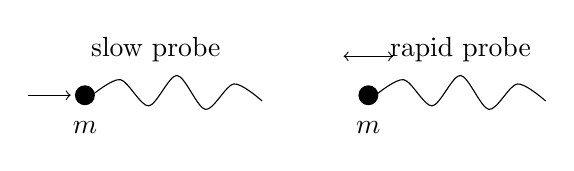
\begin{tikzpicture}[scale=0.9]
\fill (-3,0) circle (4pt);
\node at (-3,-0.45) {$m$};
\draw[smooth] plot coordinates {
(-2.9,0) (-2.5,0.22) (-2.1,-0.15) (-1.7,0.28)
(-1.3,-0.20) (-0.9,0.16) (-0.5,-0.08)
};
\draw[->] (-3.8,0) -- (-3.2,0);
\node at (-2.0,0.65) {slow probe};

\fill (1.0,0) circle (4pt);
\node at (1.0,-0.45) {$m$};
\draw[smooth] plot coordinates {
(1.1,0) (1.5,0.22) (1.9,-0.15) (2.3,0.28)
(2.7,-0.20) (3.1,0.16) (3.5,-0.08)
};
\draw[<->] (0.65,0.55) -- (1.35,0.55);
\node at (2.3,0.65) {rapid probe};
\end{tikzpicture}
\caption{慢速探測會使核心和附著其上的柔軟材料一起運動；快速探測在最初主要測得核心的響應。}
\end{figure}

這是經典物理的類比。由於系統的不同部分在不同頻率下有時間參與響應，因此推得的質量會依所施加作用力的頻率而變。

強子內的夸克周圍有強烈交互作用的膠子物質，也有其他組分。如果能非常緩慢地拉動夸克，整個強子都會跟著響應。此時所感受到的慣性將與核子質量同量級，
\begin{equation}
m_N\sim930\text{--}940\,\mathrm{MeV}.
\end{equation}
如果夸克受到猛烈撞擊，並在極短時間內受到探測，最初的響應則與通常賦予輕夸克、數值小得多的質量參數有關；在此處採用的估計中，約為
\begin{equation}
m_{u,d}\sim5\text{--}10\,\mathrm{MeV}
\end{equation}

因此，``夸克的質量''這個說法必須說明探測的尺度。輕柔的低頻擾動會帶動延展的複合體；猛烈的高頻擾動最初則只解析出其中小得多的部分。這個類比並非重整化的推導，但能說明為什麼描述粒子的參數會依據測量時所涉及交互作用的頻率和波長而變。這種依尺度而變的參數稱為跑動參數或跑動常數。

\begin{classroomqa}
\audiencequestion{這種依頻率而變的質量，是否只是重述像\(\Delta x\,\Delta t\)這樣的不確定性關係？\lecturetimestamp{01:33:32}}
\lecturerresponse{不是。這個例子本身就是一種經典現象。柔軟物體上附著的小質量，在快速作用力下和緩慢作用力下會以不同方式加速，因為附著材料中有不同部分來得及響應。}
\end{classroomqa}

\begin{classroomqa}
\audiencequestion{前面討論電子電荷時，是否也涉及同樣的尺度依賴性？\lecturetimestamp{01:34:04}}
\lecturerresponse{是的。一般而言，用來描述粒子的參數會依探測時所涉及交互作用的頻率和波長而變，這些參數稱為跑動常數。}
\end{classroomqa}

\begin{classroomqa}
\audiencequestion{賦予夸克的分數電荷，也需要作同樣的限定嗎？\lecturetimestamp{01:34:36}}
\lecturerresponse{需要。必須仔細定義夸克的電荷是什麼意思。在這個層次上，夸克電荷是相對於質子電荷而言；更完整的定義則留待另行討論。}
\end{classroomqa}

\editorialnote{固定的分數電荷量子數，與依尺度而變的交互作用耦合是不同的。耦合常數的跑動不會改變\(+\tfrac23\)或\(-\tfrac13\)味標籤本身。}

\begin{classroomqa}
\audiencequestion{為什麼顏色記帳總是使用一個夸克和一個反夸克？為什麼不能由兩個夸克構成相應的組合？\lecturetimestamp{01:34:55}}
\lecturerresponse{這是個重要問題，但答案要留待下一段有關允許的顏色組合與禁閉的討論。}
\end{classroomqa}

\begin{classroomqa}
\audiencequestion{如果無法孤立單個夸克，又是如何推斷出分數電荷、顏色和夸克模型的？\lecturetimestamp{01:35:17}}
\lecturerresponse{這個圖像是從許多線索和表面上的矛盾中逐步形成的。強子的規律暗示了夸克組分；Delta態則暴露出它與費米統計之間的衝突；夸克永久受到禁閉，則是另一個奇特的事實。夸克模型在1960年代初期提出，南部陽一郎很早就提出了重要的顏色概念，而許多物理學家在隨後約十年間共同拼湊並檢驗出完整架構。這並非單一觀測或某一個人的成果。}
\end{classroomqa}

\begin{classroomqa}
\audiencequestion{為什麼膠子只有八種，而不是表面上九種顏色--反顏色組合？\lecturetimestamp{01:37:24}}
\lecturerresponse{為什麼對角線總和不構成額外膠子的詳細解釋，留待之後說明。}
\end{classroomqa}

\begin{classroomqa}
\audiencequestion{這段量子色動力學的討論忽略了電子嗎？\lecturetimestamp{01:37:33}}
\lecturerresponse{是的。這裡先單獨討論量子色動力學，就像討論量子電動力學時可以暫時不談夸克一樣。最後仍須將這些分開的部分整合成更大的架構，納入夸克、電子、光子及其他粒子。這項整合有些部分已完成，有些部分尚未完成。物理學常透過先分離子系統、理解它，再把各部分整合起來而逐步發展。}
\end{classroomqa}